\chapter{Úvod}
\label{cha:introduction}

Steganografie je obor zabývající se skrýváním informace takovým způsobem, aby
nebylo možné zjistit její přítomnost. Důvod pro takovéto skrývání informace
může být zajištění bezpečnosti před nějakou třetí stranou pro kterou není
informace určena. Steganografie se dnes dělí na tradiční a~digitální.
V~digitální steganografii je velké množství typů dat do kterých je možné
vkládat utajované informace a~digitální zvuk je jedním z~nich.

V~oblasti digitální zvukové steganografie je dostupné velké množství kvalitní
literatury popisující teoretické fungování metod, kterými se jednotlivé
publikace zabývají. Je však těžké najít konkrétní implementace popisovaných
metod i~přesto, že autoři je implementovali pro získání výsledků. Proto je
hlavním cílem této práce vytvořit softwarovou knihovnu a~program
v~programovacím jazyce Python, aby měl kdokoliv možnost pracovat na výzkumu
v~této vědecké disciplíně. Někdy totiž nestačí pouze algoritmický popis různých
metod pro pochopení jejich fungování. Implementace v~konkrétním programovacím
jazyce nám přináší formalismus, který umožňuje snazší pochopení. Chtěl bych
proto touto prací přispět v~této oblasti tím, že bude přístupnější pro širší
veřejnost.

V~následujících kapitolách této práce je shrnut současný stav tohoto oboru,
jsou vysvětleny cíle a~technické prostředky použité k~jejich dosažení
a~zhodnoceny dosažené výsledky. V~kapitole~\ref{cha:digital-steganography}
\uv{Význam steganografie a~přehled existujících metod digitální zvukové
steganografie} jsou do hloubky popsány steganografické metody vybrané pro
implementaci a~některé další používané. Kapitola~\ref{cha:library-design}
popisuje proč byl vybrán programovací jazyk Python a~použité knihovny. Je zde
také popsána struktura balíčků pro Python a~steganografické metody které byly
vybrány pro implementaci včetně popisu vlastní metody.
Kapitola~\ref{cha:implementation} je zaměřená na popis rozvržení kódu
a~implementaci steganografických metod. Na konci kapitoly je popsán způsob
vyhodnocení kvality metod, výsledky testování a~srovnání metod. Na závěr
kapitola~\ref{cha:conclusion} obsahuje shrnutí výsledků práce a~vyhlídky do
budoucna.


\chapter{Digitální steganografie}
\label{cha:digital-steganography}

Tato kapitola představí steganografii obecně a~její klasifikace. Poté bude
stručně popsán způsob jakým se dnes reprezentuje digitální zvuk. Dále budou
vysvětleny vlastnosti na základě kterých budou metody hodnoceny a~srovnávány
včetně způsobu jejich ověření. Závěr této kapitoly se bude věnovat existujícím
steganografickým metodám včetně jejich možných modifikací.

\section{Základní definice a~klasifikace}
\label{sec:definitions}

Steganografie je praktika skrývání informace s~cílem zakrýt její samotnou
existenci a~ne jen znemožnit její čtení
\cite{AlSabhany2020}\cite{Anderson1998}\cite{Djebbar2012}\cite{Dutta2020}.
Původ této praktiky se vrací až do antiky -- vyrytím písma do destičky, která
se následně zalila voskem; ve středověké Evropě položením papíru nebo dřevěné
šablony na nevinně vypadající text, čímž zvýrazní tajnou zprávu. Steganografie
se tedy v~různých podobách praktikovala po tisíciletí až do dnešní počítačové
doby \cite{Anderson1998}, kdy je považována za podobor zabezpečení dat
\cite{Djebbar2012} a~více se přesouvá od tradiční k~digitální steganografii.

V~dnešním světě se stalo zabezpečení dat zájmem všech a~steganografie jako
proces ukrývání zprávy do jiného typu média slouží k~ochraně před
neautorizovanými či neoprávněnými příjemci \cite{Dutta2020}. Médium do kterého
je informace skrývána se nazývá nosič a~může být různých typů, jako například
obrázek, audio, video, IP datagram \cite{Dutta2020}, text a~mnoho dalších.
Hierarchickou klasifikaci je možné vidět na obrázku
\ref{pic:steganography-classification}.

\begin{figure}[hbt]
    \centering
    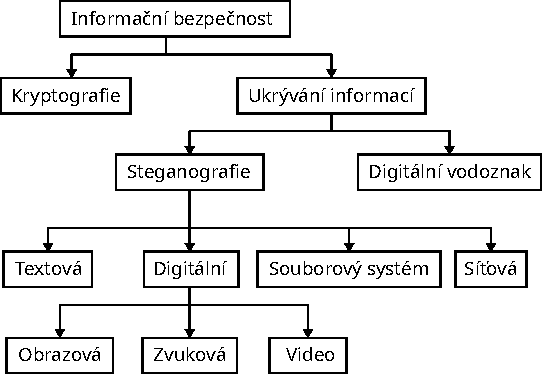
\includegraphics[width=0.8\textwidth]{obrazky/steganography-classification.pdf}
    \caption{Klasifikace oboru informační bezpečnosti a~steganografie.
    Přeloženo z~\cite{Elshoush2022}.}
    \label{pic:steganography-classification}
\end{figure}

Pokud je nosičem počítačový soubor, pak se může nazývat \textit{krycí soubor},
tyto dva názvy jsou však často zaměnitelné. Každý typ nosiče má svoji oblast
výzkumu, která se jej týká. Některé steganografické metody používané u~různých
typů nosičů jsou konceptuálně stejné a~v~praxi se aplikují podobným způsobem.
Tato práce se však bude zabývat pouze metodami použitelnými pro digitální
audio a~proto následující podkapitola vysvětlí způsob jakým se reprezentuje
zvuk v~digitální formě.

\section{Reprezentace a~způsob uložení digitálního zvuku}
\label{sec:digital-sound-representation}

V~reálném světě se zvuk vyskytuje jako vibrace materiálu při frekvenci
slyšitelné člověkem, která se pohybuje mezi 10\,Hz a~20\,000\,Hz
\cite{Swanson1998}. Zvuk je ve skutečném světě spojitý signál -- má nekonečný
počet hodnot -- a~je tedy definován všude. Aby bylo možné se zvukem pracovat
digitálně, je nutné převést jej do diskrétní formy, která má konečný počet
hodnot. Toho je možné docílit vzorkováním signálu na určité vzorkovací
frekvenci a~poté kvantováním \cite{Cernocky2021}. Posledním krokem pro převod
spojitého signálu na digitální, je kódování. Tyto tři procesy tvoří systém,
který se nazývá \textit{pulzně-kódová modulace}~(PCM) \cite{Oliver1948}, který
je neopominutelným základem pro práci s~digitálním audiem.

\subsection*{Vzorkování}
\label{sub:sampling}

Vzorkování probíhá tak, že se každá sekunda spojitého signálu rozdělí na tolik
bodů, kolik udává vzorkovací frekvence. V~každém bodě se zjistí amplituda ve
stejném bodě spojitého signálu a~ta se stane jeho hodnotou. Rozdíl mezi
spojitým a~navzorkovaným signálem je vidět na
obrázku~\ref{pic:continuous-vs-sampled-signal}. Aby nedošlo ke ztrátě
informace, je nutné dodržet Nyquist-Shannonův vzorkovací teorém, podle kterého
musí být nejvyšší frekvence přítomná v~signálu maximálně polovina vzorkovací
frekvence \cite{Shannon1949}. Nejčastěji používané vzorkovací frekvence jsou
44\,100\,Hz a~48\,000\,Hz. Nejvyšší frekvence, které lze na těchto vzorkovacích
frekvencích reprezentovat bez ztráty informace jsou příslušně 22\,050\,Hz
a~24\,000\,Hz.

\pgfplotsset{
    standard/.style={
        axis x line=middle,
        axis y line=middle,
        enlarge x limits=0.15,
        enlarge y limits=0.15,
        every axis x label/.style={
            at={(current axis.right of origin)},
            anchor=north west
        },
        every axis y label/.style={
            at={(current axis.above origin)},
            anchor=north east
        },
        every axis plot post/.style={
            mark options={fill=white}
        }
    }
}

\begin{figure}[hbt]
    \centering
    \begin{subfigure}[b]{0.5\linewidth}
        \centering
        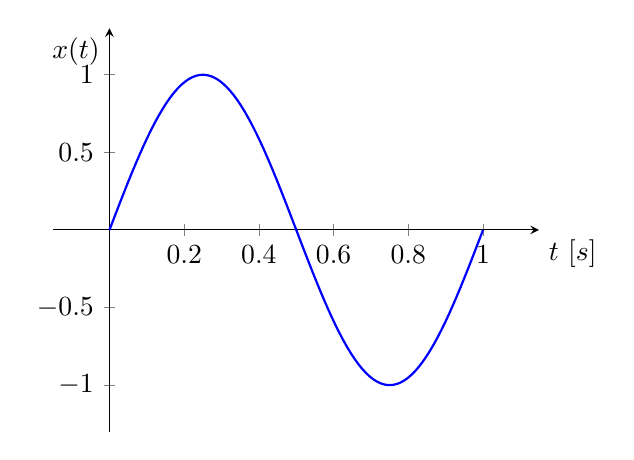
\begin{tikzpicture}
            \begin{axis}[%
                standard,
                scale=0.9,
                domain = 0:1,
                samples = 100,
                xlabel = {$t~[s]$},
                ylabel = {$x(t)$}]
                \addplot[blue,thick] {sin(2*180*x)};
            \end{axis}
        \end{tikzpicture}
    \end{subfigure}%
    \begin{subfigure}[b]{0.5\linewidth}
        \centering
        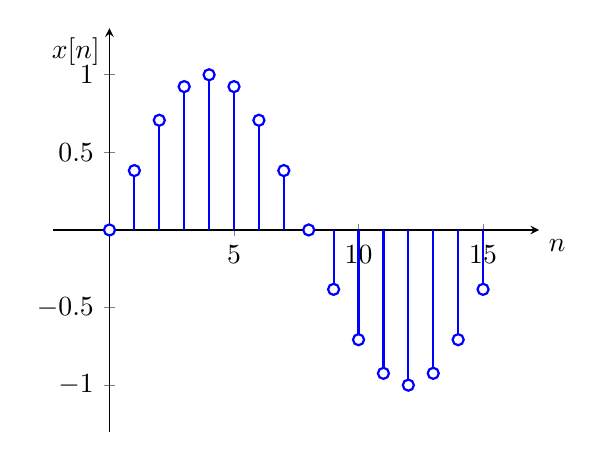
\begin{tikzpicture}
            \begin{axis}[%
                standard,
                scale=0.9,
                domain = 0:15,
                samples = 16,
                xlabel = {$n$},
                ylabel = {$x[n]$}]
                \addplot+[ycomb,blue,thick] {sin(2*180*x/16)};
            \end{axis}
        \end{tikzpicture}
    \end{subfigure}
    \caption{Spojitý signál (vlevo) a~navzorkovaný signál (vpravo) vzorkovaný
    na frekvenci 16\,Hz}
    \label{pic:continuous-vs-sampled-signal}
\end{figure}

\subsection*{Kvantování}
\label{sub:quantization}

Pro převedení spojitého signálu na digitální nestačí pouze vzorkování.
Vzorkování diskretizuje časovou komponentu spojitého signálu na pevně daný
počet vzorků za jednotku času, ale nijak neovlivňuje hodnoty, kterých
jednotlivé vzorky mohou nabývat. Kvantování je proces diskretizace hodnot
zaokrouhlováním k~předem určeným hodnotám \cite{Oliver1948}. Hodnoty nebo také
hladiny, ke kterým se zaokrouhluje jsou dané počtem použitých bitů. Vyšší počet
bitů vede ke zlepšení kvality, protože zaokrouhlené hodnoty jsou blíže jejich
původním. Tento jev lze vidět na obrázku \ref{pic:quantization}. Proces
kvantování vždy zavede do výsledného signálu takzvaný \textit{kvantizační šum}
\cite{Oliver1948}, protože převedení reálných čísel na digitální není exaktní.
Tento šum je rozdílem původního signálu a~kvantovaného signálu. Použití menšího
počtu bitů způsobí, že kvantizační šum bude výraznější, ale výsledný signál
bude mít menší velikost. Pro kvalitní audio se dnes nejčastěji používá alespoň
16~bitů.

\begin{figure}[hbt]
    \centering
    \begin{subfigure}[b]{0.5\linewidth}
        \centering
        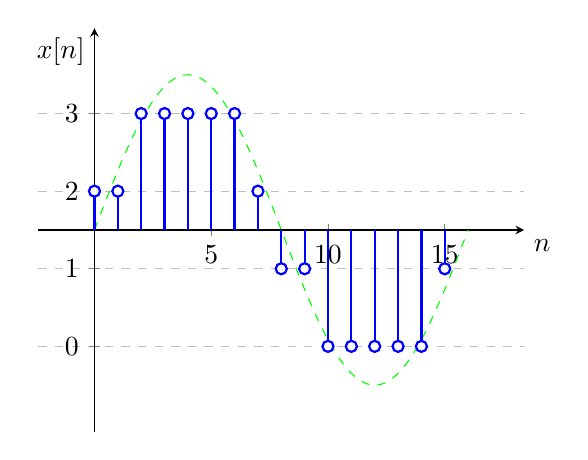
\begin{tikzpicture}
            \begin{axis}[%
                standard,
                scale=0.9,
                domain = 0:16,
                xlabel = {$n$},
                ylabel = {$x[n]$},
                ytick = {-1.5, -0.5, 0.5, 1.5},
                yticklabels = {$0$, $1$, $2$, $3$},
                ymajorgrids = true,
                grid style = dashed,
                ]
                \addplot[green,dashed,samples=100] {2*sin(2*180*x/16)};
                \addplot+[ycomb,blue,thick,mark=*] coordinates{
                    (0,0.5)(1,0.5) (2,1.5) (3,1.5) (4,1.5) (5,1.5) (6,1.5)
                    (7,0.5) (8,-0.5) (9,-0.5) (10,-1.5) (11,-1.5) (12,-1.5)
                    (13,-1.5) (14,-1.5) (15,-0.5)
                };
            \end{axis}
        \end{tikzpicture}
    \end{subfigure}%
    \begin{subfigure}[b]{0.5\linewidth}
        \centering
        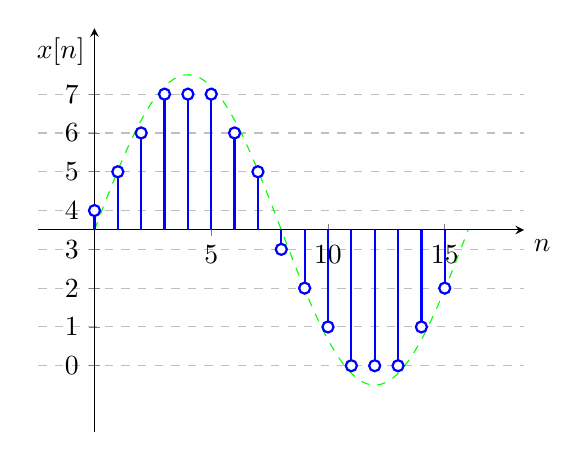
\begin{tikzpicture}
            \begin{axis}[%
                standard,
                scale=0.9,
                domain = 0:16,
                xlabel = {$n$},
                ylabel = {$x[n]$},
                ytick = {-3.5, -2.5, -1.5, -0.5, 0.5, 1.5, 2.5, 3.5},
                yticklabels = {$0$, $1$, $2$, $3$, $4$, $5$, $6$, $7$},
                ymajorgrids = true,
                grid style = dashed,
                ]
                \addplot[green,dashed,samples=100] {4*sin(2*180*x/16)};
                \addplot+[ycomb,blue,thick,mark=*] coordinates{
                    (0,0.5)(1,1.5) (2,2.5) (3,3.5) (4,3.5) (5,3.5) (6,2.5)
                    (7,1.5) (8,-0.5) (9,-1.5) (10,-2.5) (11,-3.5) (12,-3.5)
                    (13,-3.5) (14,-2.5) (15,-1.5)
                };
            \end{axis}
        \end{tikzpicture}
    \end{subfigure}
    \caption{Signál z~obrázku \ref{pic:continuous-vs-sampled-signal}
    vzorkovaný na frekvenci~16\,Hz a~kvantovaný na 2~bitech (vlevo) a~4~bitech
(vpravo)}
    \label{pic:quantization}
\end{figure}

Na závěr, pro uložení a~přenos digitálních signálů musí být vzorky zakódovány.
Nejjednodušší způsob pro zakódování kvantovaných hodnot je převedením na
binární čísla. Jednotlivé jedničky a~nuly pak mohou při přenosu reprezentovat
přítomnost pulzu~(1) a~nepřítomnost pulzu~(0). Tento systém, který obsahuje
vzorkování, kvantování a~kódování, se nazývá \textit{pulzně-kódová
modulace}~(PCM) \cite{Oliver1948}. Pulzně-kódová modulace je důležitá obecně
pro zpracování digitálních signálů, ale i~pro účely této práce, protože ji
využívá zvukový formát \textit{Waveform Audio File Format}, který je popsán
v~následující podsekci.

\subsection*{Formáty digitálního zvuku}
\label{sub:digital-audio-formats}

Digitálních audio formátů je velké množství, každý se svými odlišnými
vlastnostmi. Hlavní kategorie na které se digitální zvukové formáty dělí jsou
\textit{nekomprimované} a~\textit{komprimované} -- ty se ještě dělí na formáty
se ztrátovou a~bezeztrátovou kompresí. Příklady některých známých formátů jsou
v~tabulce \ref{tab:audio-formats}.

\begin{table}[H]
    \vskip6pt
    \caption{Tabulka známých zvukových formátů}
    \vskip6pt
    \centering
    \begin{tabular}{lll}
        \toprule
        Nekomprimovaný & \multicolumn{2}{c}{Komprimovaný} \\
        \cmidrule(r){2-3}
                       & Bezeztrátový & Ztrátový \\
        \midrule
        WAV  & FLAC & MP3 \\
        AIFF & ALAC & AAC \\
        RAW  &      & OGG Vorbis \\
             &      & Opus \\
             &      & WebM \\
        \bottomrule
    \end{tabular}
    \label{tab:audio-formats}
\end{table}

\textit{Waveform Audio File Format} (dále jen WAV) je proprietární formát pro
digitální audio vytvořený firmami Microsoft a~IBM. Je široce rozšířený a~není
k~němu potřeba žádná licence. Tento formát je nástavbou generického
multimediálního formátu \textit{Resource Interchange File Format} (RIFF).
Konkrétní typ pulzně-kódové modulace, který WAV formát nejčastěji používá je
lineární pulzně-kódová modulace (LPCM) \cite{RFC2361} -- kvantovací úrovně mají
mezi sebou rovnoměrné rozestupy \cite{LPCM}. Může ale používat i~jiné typy
kódování, jako \textit{IEEE Float} nebo komprimované \textmu-Law a~A-Law
\cite{RFC2361}.

V~roce 2020 provedli AlSabhany, Ali, Ridzuan a~další \cite{AlSabhany2020}
systematické srovnání 134~publikací zabývající se digitální zvukovou
steganografií a~zjistili, že 84\%~z~nich používalo formát WAV jako nosič. Za
účelem jednoduššího srovnávání metod bude tato práce pracovat pouze s~formátem
WAV.

\section{Digitální zvuková steganografie}
\label{sec:digital-audio-steganography}

Poslední dobou se začaly objevovat nové směry založené na steganografických
přístupech pro zajištění bezpečnosti a~utajení dat které by v~kombinaci
s~konvenčními bezpečnostními technikami mohly vést k~lepším výsledkům
\cite{Djebbar2012}. Jedna z~konvenčních bezpečnostních technik kombinovaných se
steganografií je kryptografie. Zatím co steganografie se zabývá ukrýváním
informace, hlavním cílem kryptografie je převést zprávu do formy, která je pro
neoprávněné osoby nečitelná \cite{AlSabhany2020}. I~když se tedy někdo pokusí
analyzovat komunikaci pro přítomnost utajené zprávy, není možné obsah rozeznat
od náhodného šumu.

Digitální zvuková steganografie má široké spektrum využití. Mezi praktické
příklady patří: monitorování reklam v~rádiu, indexování video zpráv, použití
všude tam, kde není možné použít šifrování, zachování soukromí jednotlivce,
utajená komunikace mezi vojenskými rozvědkami nebo bezpečnostními
složkami~\cite{Dutta2020}.

Dalším často používaným pojmem spojeným se steganografií je vodoznak. Vodoznaky
se používají pro vložení informací o~původu, vlastnictví, či autorských právech
dat \cite{Djebbar2012}\cite{Dutta2020}\cite{Swanson1998}. Hlavní vlastností
vodoznaku je, že by nemělo být možné jej odstranit bez poškození nosného média.
Proto u~audia nesmí být součástí hlavičky souboru nebo být přenášen zvlášť, ale
být jeho součástí a~musí být nedetekovatelný. Musí být také odolný proti
transformaci signálu například při přenosu audia nebo převedení do formátu,
který používá ztrátovou kompresi \cite{Swanson1998}. Velice známým příkladem
jsou vodoznaky na bankovkách nebo \textit{žluté tečky} v~tiskárnové
steganografii -- známé také jako \textit{yellow dots} -- které barevné tiskárny
tisknou na každý list. Tyto tečky obsahují zakódované sériové číslo tiskárny
a~čas tisku \cite{Dutta2020}. Pokud je vodoznak použit pro ochranu
intelektuálního vlastnictví, pak se ještě rozlišuje mezi vodoznakem a~otiskem.
Vodoznakem se značí všechny objekty stejně, ale otisk se může měnit například
pro každého zákazníka pro jeho pozdější identifikaci. To může být užitečné
pokud poruší licenční podmínky například sdílením zakoupené hudby
\cite{Swanson1998}.

\section{Vlastnosti a~jejich ověřování}
\label{sec:method-properties}

Aby bylo možné jednotlivé metody srovnávat mezi sebou, je nutné určit
vlastnosti podle kterých budou hodnoceny. Těch může být mnoho, ale různí autoři
steganografických publikací se shodují, že nejvýznamnějšími vlastnostmi jsou
\textit{robustnost}, \textit{kapacita} a~\textit{nepostřehnutelnost}
\cite{AlSabhany2020}\cite{Djebbar2012}\cite{Dutta2020}. Tyto tři vlastnosti je
možné si představit jako trojúhelník s~každou vlastností v~jednom rohu, jak je
vidět na obrázku \ref{pic:method-property-triangle}. Důvodem je fakt, že není
možné dosáhnout vysoké úrovně všech tří vlastností zároveň \cite{Dutta2020}.
Zvýšení kvality jedné z~vlastností vždy vede ke snížení kvality alespoň jedné
zbývající \cite{AlSabhany2020}\cite{Djebbar2012}. V~následujících podsekcích
budou popsány jednotlivé vlastnosti podrobněji. Bude také několikrát použit
pojem \textit{stego soubor}, což je soubor, který vznikne použitím určité
steganografické metody pro ukrytí zvolené informace do krycího souboru.

\begin{figure}[hbt]
    \centering
    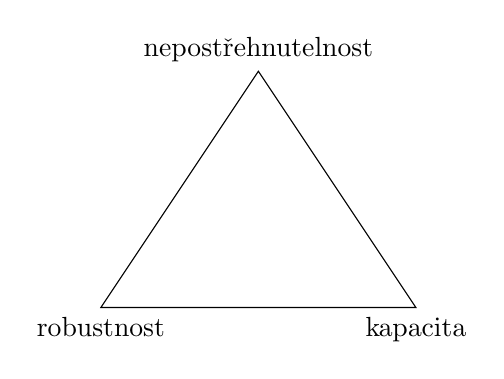
\begin{tikzpicture}
        \draw (0,0) coordinate[label=below:robustnost] --
              (4,0) coordinate[label=below:kapacita] --
              (2,3) coordinate[label=above:nepostřehnutelnost] --
              cycle;
    \end{tikzpicture}
    \caption{Trojúhelník se třemi nejvýznamnějšími vlastnostmi
    steganografických metod}
    \label{pic:method-property-triangle}
\end{figure}

\subsection*{Robustnost}
\label{sub:robustness}

Robustnost indikuje odolnost metody proti úmyslným či neúmyslným modifikacím
skrytých informací \cite{AlSabhany2020}\cite{Dutta2020}. Míru robustnosti lze
hodnotit na základě množství skryté informace, která zůstane nezměněná po
různých úpravách stego souboru. Podle \cite{Djebbar2012} mohou tyto modifikace
být:

\begin{itemize}
    \item zesílení amplitudy -- může poškodit skryté informace
    \item filtrování -- skryté informace mohou být odstraněny filtrací určitého
        pásma
    \item překvantování -- snížením počtu bitů a~zpětné překvantování na
        původní hodnotu zavede nejen kvantizační šum, ale může být poškozena
        nebo odstraněna skrytá informace
    \item převzorkování -- podobná situace jako u~překvantování, snížení
        vzorkovací frekvence způsobí ztrátu informace
    \item přidání šumu -- šum může skrytá data zamaskovat nebo poškodit
    \item překódování -- skrytá informace může být poškozena převedením stego
        souboru do formátu, který používá ztrátovou kompresi
\end{itemize}

Robustnost metody je obzvlášť důležitá pro tvorbu vodoznaku popsaného
v~podsekci~\ref{sec:digital-audio-steganography}. Vodoznak musí být schopen
odolat výše zmíněným modifikacím, aby bylo možné správně identifikovat jeho
vlastníka \cite{Swanson1998}.

\subsection*{Kapacita}
\label{sub:capacity}

Kapacita udává množství informace, které je možné do nosiče zakódovat a~úspěšně
dekódovat \cite{Dutta2020}\cite{Djebbar2012}. Kapacitu metody je možné vyjádřit
bitech za sekundu ($bps$ nebo také $b/s$) nebo jako procentuální poměr
velikosti skryté informace k~velikosti nosiče
\cite{AlSabhany2020}\cite{Dutta2020}. Výhodou zvukových steganografických metod
je velká velikost souborů, což umožňuje skrýt větší množství informací. Zároveň
je možné ukládat informace do nevyužitých polí v~hlavičkách souborů
\cite{Dutta2020}.

\subsection*{Nepostřehnutelnost}
\label{sub:imperceptibility}

Tato vlastnost vyjadřuje podobnost stego souboru a~krycího souboru a~je spojená
s~detekovatelností přítomnosti skryté informace \cite{AlSabhany2020}. Úroveň
nepostřehnutelnosti je možné měřit pomocí \textit{perceptual evaluation of
speech quality} (PESQ) testu. Hodnota~4,5 znamená, že naměřený stego soubor je
totožný s~krycím souborem. Hodnota~1 indikuje maximální degradaci kvality.
Další způsob pro porovnání rozdílů dvou signálů je \textit{segmentový poměr
signálu k~šumu} (SegSNR) \cite{Djebbar2012}. V~již zmíněné studii z~roku~2020
\cite{AlSabhany2020} zjistili autoři, že nejpoužívanější metodou napříč
analyzovanými publikacemi byl globální \textit{poměr signálu k~šumu} (SNR)
a~dále \textit{špičkový poměr signálu k~šumu} (PSNR).

Zvukové steganografické metody mají tu nevýhodu, že lidské zvukové ústrojí je
velmi citlivé. Přesto má nedostatky, které je možné využít, jako například
maskování tónu, který následuje po hlasitém impulzu. Dalším příkladem je
maskování informace, která je zakódovaná ve frekvenci zvuku, který se nachází
poblíž \cite{Dutta2020}.

\section{Existující řešení}
\label{sec:existing-methods}

V~této podkapitole bude popsáno několik existujících metod digitální zvukové
steganografie. Popis každé metody bude obsahovat její princip a~silné a~slabé
stránky. Každý popis bude obsahovat konkrétní způsob jakým je možné zakódovat
a~dekódovat informace danou metodou. Na závěr každého popisu metody budou
diskutovány možnosti modifikace metody pro zlepšení nějaké ze steganografických
vlastností.

\subsection*{Metoda nahrazení nejméně významného bitu}
\label{sub:lsb}

Metoda využívající nahrazení nejméně významného bitu (anglicky \textit{least
significant bit substitution}, dále jen LSB) je nejjednodušší metodou pro
vkládání informací do nosiče. Principem této metody je nahrazení nejméně
významného bitu v~nosiči za bit ukrývané informace \cite{Dutta2020}. Princip
kódování pomocí této metody je vizualizován na obrázku \ref{pic:lsb-diagram}.

\begin{figure}[hbt]
    \centering
    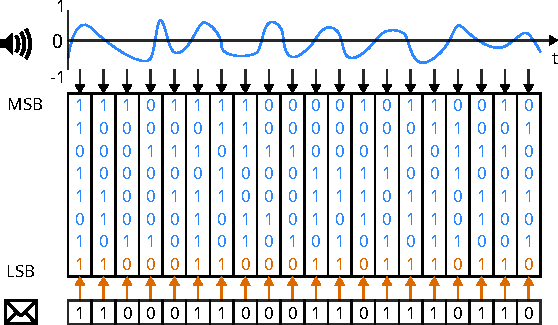
\includegraphics[width=0.8\textwidth]{obrazky/lsb-diagram.pdf}
    \caption{Ukládání informačních bitů do nejméně významného bitu krycího
    signálu. Upraveno z~\cite{Djebbar2012}.}
    \label{pic:lsb-diagram}
\end{figure}

Tato metoda se vyznačuje velmi vysokou kapacitu \cite{Djebbar2012}
a~jednoduchou implementací. Kapacita této metody je přímo úměrná počtu
a~bitovou hloubkou vzorků nosiče. Je také vhodná pro kombinaci s~dalšími
steganografickými technikami \cite{Djebbar2012} jako je šifrování nebo
komprese. Hlavní nevýhodou této metody je její nízká robustnost. Informace
ukryté LSB metodou je velmi jednoduché poškodit triviálními úpravami stego
souboru jako je například zesílení, filtrace, přidání šumu, ztrátová komprese
\cite{Djebbar2012}, převzorkování nebo překvantování. Robustnost této metody
a~odolnost proti některým z~těchto modifikací je možné zvýšit vkládáním do jiné
bitové úrovně než je poslední \cite{Djebbar2012}.

Nemodifikovaná LSB metoda není příliš bezpečná, neboť je možné jednoduše vyčíst
hodnoty určité bitové úrovně a~tím odhalit ukryté informace \cite{Djebbar2012}.
Pro lepší ukrytí informací je možné ukládat bity do náhodných vzorků
a~náhodných úrovní v~nich \cite{Dutta2020}. Bezpečnost LSB metody je možné
zvýšit šifrováním ukrývaných informací. Ukrývaná data je vhodné nejprve
zkomprimovat například Lempel-Ziv-Welch (LZW) kompresí. Poté je možné je
zašifrovat vybraným šifrovacím algoritmem. Vhodným algoritmem pro symetrické
šifrování je \textit{Advanced Encryption Standard} (AES, česky standard
pokročilého šifrování). Pro asymetrické šifrování je vhodný algoritmus
Rivest-Shamir-Adleman (RSA) \cite{Dutta2020}.

Kapacitu LSB metody je možné zvýšit například ukládáním do více bitových úrovní
za sebou v~jednotlivých vzorcích. Tato modifikace však produkuje šum, který je
lidské ucho schopno zachytit. Lepším způsobem jak zvýšit kapacitu je vkládáním
do 4~nejnižších bitových úrovní pomocí algoritmu \textit{nahrazení nejmenší
chybou} (anglicky minimum-error replacement) a~rozprostření chyby do
následujících 4~vzorků. Tato modifikace zvyšuje kapacitu LSB metody o~33\%
zatímco poměr signálu k~šumu je nižší než u~nemodifikované metody se stejným
počtem použitých bitů \cite{Cvejic2002}.

\subsection*{Metoda skrývání pomocí ozvěny}
\label{sub:echo-hiding}

Steganografická metoda ukrývání informací pomocí ozvěny (anglicky echo hiding)
funguje na principu přidání ozvěny do krycího média \cite{Djebbar2012}. Tato
metoda má vyšší robustnost vůči filtrování, převzorkování, či ztrátové
kompresi. Lidské sluchové ústrojí má široký dynamických rozsah výkonu
a~frekvence, ale přesto je možné využít nedostatků, jako je maskování tichých
zvuků hlasitějšími \cite{Gruhl1996}. Nevýhodou této metody je zkreslení
způsobené přidáním ozvěny do krycího média, které je srovnatelné s~rozdílem
poslechu audia ve sluchátkách a~přes reproduktory, kde se zvuk odráží od stěn
v~místnosti. Při vhodném nastavení parametrů je možné docílit výborné
nepostřehnutelnosti \cite{Gruhl1996}. Tato metoda má dostatečnou míru
robustnosti a~je tedy vhodná pro zakódování vodoznaku do krycího média. Vhodné
nastavení parametrů docílí velmi nízké pravděpodobnosti odhalení či odstranění
vodoznaku neoprávněnou osobou \cite{Gruhl1996}. Po přidání ozvěny si stego
médium udrží stejné statistické a~percepční vlastnosti \cite{Djebbar2012}.

Pro implementaci této metody se krycí médium rozdělí na segmenty do kterých se
bity ukrývané informace zakódují vytvořením ozvěny daného segmentu. Pro
rozlišení hodnoty bitu se použije jiná míra zpoždění pro logickou~1
a~logickou~0. Kódování probíhá konvolucí segmentu a~konvolučním jádrem pro
příslušný bit. Jednotlivé segmenty se následně spojí a~přidají ke krycímu médiu
\cite{Gruhl1996}. V~praxi je ale výhodnější provést konvoluci krycího média
s~oběma konvolučními jádry a~použít bity ukrývané informace jako masku, která
určí které segmenty ponechat a~přidat ke krycímu médiu \cite{Gruhl1996}. Pro
snížení míry zkreslení na rozmezí segmentů je vhodné vyhladit změnu mezi
hodnotou~0~a~1 \cite{Tekeli2017}. Příklad ozvěn, které vniknou použitím masky
bez vyhlazení jsou na obrázku \ref{pic:echo-single-kernel-echo}. Příklad ozvěn,
které vniknou použitím masky s~vyhlazením jsou na obrázku
\ref{pic:echo-single-kernel-echo-smooth}.

\begin{figure}[hbt]
    \centering
    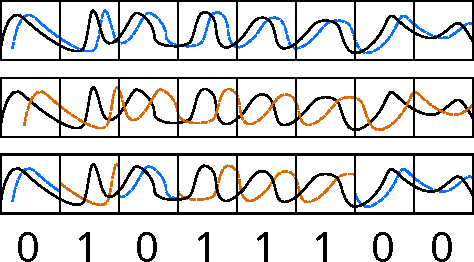
\includegraphics[width=0.8\textwidth]{obrazky/echo-diagram.pdf}
    \caption{Ozvěny vzniklé konvolucí s~konvolučními jádry pro jednu ozvěnu bez
    vyhlazení.}
    \label{pic:echo-single-kernel-echo}
\end{figure}

\begin{figure}[hbt]
    \centering
    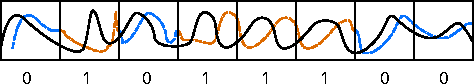
\includegraphics[width=0.8\textwidth]{obrazky/echo-smoothed.pdf}
    \caption{Ozvěny vzniklé konvolucí s~konvolučními jádry pro jednu ozvěnu
    s~vyhlazením.}
    \label{pic:echo-single-kernel-echo-smooth}
\end{figure}

\subsubsection*{Ozvěna s~jedním konvolučním jádrem na bit}
\label{ssub:echo-single-kernel}

Tuto metodu poprvé představil Daniel Gruhl a~Walter Bender v~roce 1996
\cite{Gruhl1996}. Používá dvě konvoluční jádra dané rovnicí
\ref{eq:echo-single-kernel}, kde $\delta$ je Kroneckerova delta funkce, $d_i$
je zpoždění pro bit logické~0 a~logické~1 a~$\alpha$ je amplituda ozvěny
\cite{Dutta2020}.

\begin{equation}
    \label{eq:echo-single-kernel}
    h_i[n] = \delta[n] + \alpha\delta[n - d_i], i \in {0, 1}
\end{equation}

\noindent Zpožděné signály vniknou konvolucemi krycího média s~konvolučními
jádry dané rovnicí \ref{eq:echo-single-kernel-echo}, kde $s[n]$ je krycí médium
a~$h_i[n]$ je konvoluční jádro z~rovnice \ref{eq:echo-single-kernel}.

\begin{equation}
    \label{eq:echo-single-kernel-echo}
    k_i[n] = s[n] * h_i[n]
\end{equation}

\noindent Příklad ozvěn, které vniknou konvolucemi krycího média s~konvolučními
jádry jsou na obrázku \ref{pic:echo-single-kernel-echo}.

\subsubsection*{Dekódování}
\label{ssub:echo-single-kernel-decoding}

K~dekódování této metody se používá cepstrální analýza. Stego signál se rozdělí
na stejný počet segmentů jako při kódování. Poté se vypočítá jejich cepstrum,
které je definováno jako inverzní Fourierova transformace ($\mathcal{F}^-1$)
logaritmu absolutní hodnoty Fourierovy transformace ($\mathcal{F}$) signálu
\cite{Tekeli2017}. Vzorec pro získání cepstra signálu $x(t)$ je definován
rovnicí \ref{eq:cepstrum}.

\begin{equation}
    \label{eq:cepstrum}
    C = \mathcal{F}^-1(\log{|\mathcal{F}(x(t))|})
\end{equation}

Po výpočtu cepstra segmentu je možné zjistit hodnotu zakódovaného bitu
kontrolou, která hodnota na pozici $d_0$ a~$d_1$ je vyšší. Pokud je hodnota
$C(d_0)$ vyšší než $C(d_1)$, pak je hodnota bitu daného segmentu logická~0.
A~pokud je hodnota $C(d_1)$ vyšší než $C(d_0)$, pak je hodnota bitu daného
segmentu logická~1 \cite{Gruhl1996}. Příklad cepstra segmentu včetně špiček na
indexech zpoždění 100 a~110 lze vidět na obrázku \ref{pic:segment-cepstrum}.

\begin{figure}[hbt]
    \centering
    \begin{subfigure}[b]{0.5\linewidth}
        \centering
        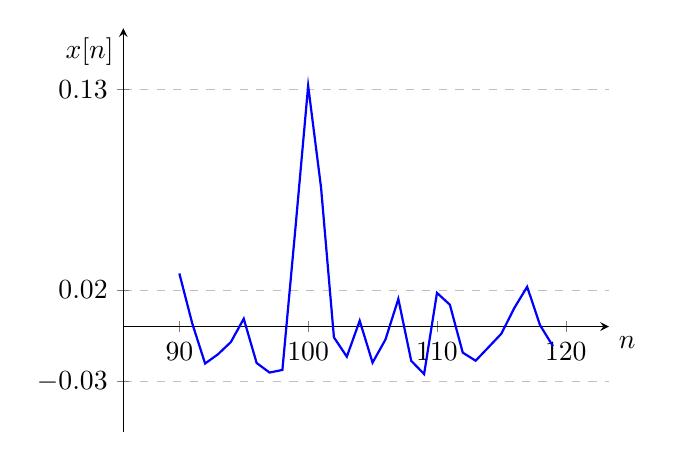
\begin{tikzpicture}
            \begin{axis}[%
                standard,
                enlarge y limits=0.2,
                scale=0.9,
                xlabel = {$n$},
                ylabel = {$x[n]$},
                scaled y ticks = false,
                y tick label style = {/pgf/number format/fixed},
                ytick = {-0.03, 0.02, 0.13},
                ymajorgrids = true,
                grid style = dashed,
                ]
                \addplot[blue,thick,samples=100] table [x={x}, y={y}] {
x y
90 0.02911713
91 0.00175175
92 -0.02027917
93 -0.01520897
94 -0.00849168
95 0.00427713
96 -0.01998557
97 -0.02522004
98 -0.02379227
99 0.05305905
100 0.13196956
101 0.07625496
102 -0.00591677
103 -0.01654206
104 0.00318564
105 -0.0197923
106 -0.00712777
107 0.01512758
108 -0.01878832
109 -0.0260548
110 0.01846125
111 0.01196165
112 -0.01430203
113 -0.01873781
114 -0.01135309
115 -0.00389159
116 0.01014747
117 0.02179004
118 0.00075464
119 -0.01072793
};
            \end{axis}
        \end{tikzpicture}
    \end{subfigure}%
    \begin{subfigure}[b]{0.5\linewidth}
        \centering
        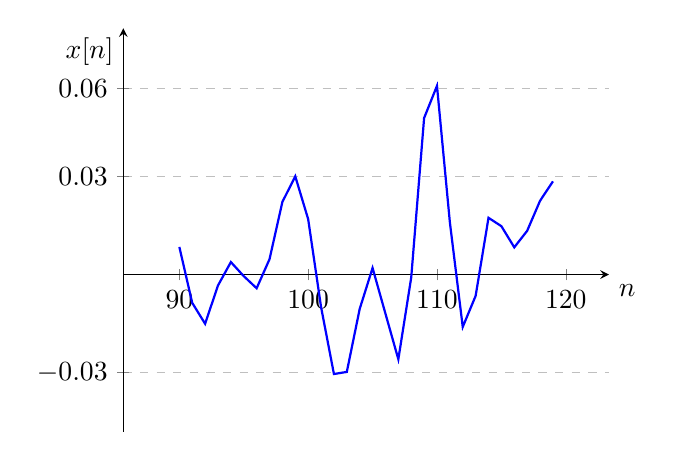
\begin{tikzpicture}
            \begin{axis}[%
                standard,
                enlarge y limits=0.2,
                scale=0.9,
                xlabel = {$n$},
                ylabel = {$x[n]$},
                scaled y ticks = false,
                y tick label style = {/pgf/number format/fixed},
                ytick = {-0.03, 0.03, 0.057},
                ymajorgrids = true,
                grid style = dashed,
                ]
                \addplot[blue,thick,samples=100] table [x={x}, y={y}] {
x y
90 0.00846854
91 -0.00866365
92 -0.01506901
93 -0.00334494
94 0.00382214
95 -0.00047939
96 -0.00419374
97 0.0046966
98 0.02226608
99 0.03008467
100 0.01698417
101 -0.00991495
102 -0.03046551
103 -0.02982553
104 -0.01053166
105 0.00202071
106 -0.01198137
107 -0.02595199
108 -0.00091994
109 0.04794415
110 0.05781149
111 0.01600666
112 -0.01603436
113 -0.00653139
114 0.01738747
115 0.014815
116 0.00833863
117 0.01340137
118 0.02259084
119 0.02855182
};
            \end{axis}
        \end{tikzpicture}
    \end{subfigure}
    \caption{Přiblížená cepstra segmentů. Levé kóduje logickou~0. Pravé kóduje
    logickou~1.}
    \label{pic:segment-cepstrum}
\end{figure}

Nevýhodou při dekódování této metody je například falešná detekce, pokud se ve
zvuku doopravdy vyskytuje ozvěna. Dále může být těžké detekovat informaci pokud
je amplituda ozvěny příliš malá a~špičky na indexech zpoždění budou tudíž
splývat s~okolím. Zesílení amplitudy zlepší míru detekce, ale zvýší také
náchylnost na neoprávněnou detekci \cite{Kim2003}.

\subsubsection*{Modifikace metody skrývání pomocí ozvěny}
\label{ssub:echo-modifications}

Pro zvýšení robustnosti a~nepostřehnutelnosti použili autoři Oh, Seok, Hong
a~Youn \cite{Oh2001} konvoluční jádro, které nejprve vytvoří ozvěnu se zápornou
amplitudou a~poté s~kladnou (anglicky bipolar echo). Zjistili, že tato
modifikace má vyšší míru robustnosti i~po překódování do ztrátového formátu
MP3. Dekódování této modifikace spočívá v~detekování špiček v~autokorelaci
výkonového cepstra. Výkonové cepstrum je podobné normálnímu cepstru a~je
definováno rovnicí \ref{eq:power-cepstrum}.

\begin{equation}
    \label{eq:power-cepstrum}
    C_p = \mathcal{F}^-1(\log{|\mathcal{F}(x(t))|}^2)
\end{equation}

O~2~roky později publikovali autoři Kim a~Choi \cite{Kim2003} způsob jak znovu
zvýšit robustnost pomocí konvolučního jádra se dvěma ozvěnami posunutými vpřed
i~vzad (anglicky backward-forward echo). Později publikovali autoři Wu a~Chen
\cite{Wu2006} modifikaci ozvěnové metody kombinující již popsané modifikace. Ta
používá konvoluční jádro pro vytvoření celkem čtyř ozvěn. Dvě jsou posunuté
vzad a~dvě vpřed přičemž obě strany mají ozvěnu s~kladnou a~zápornou
amplitudou. Autoři porovnávali tuto modifikaci s~výše popsanými variantami této
metody a~ve všech testech měla vyšší poměr úspěšně dekódovaných bitů a~zároveň
také vyšší poměr signálu k~šumu než ostatní varianty.

\subsection*{Metoda rozprostřeného spektra}
\label{sub:dsss}

Metoda rozprostřeného spektra byla nejprve vytvořena jako metoda pro zvýšení
spolehlivosti přenosu dat a~zajištění doručení informací. Ze stejných důvodů se
rozprostření spektra používá i~ve steganografii. Princip této metody spočívá
v~opakování informačních bitů $n$-krát podle čipové rychlosti (anglicky
\textit{chip rate}). Ta určuje kolika bity bude kódován každý informační bit.
\cite{AlSabhany2020}. Dále popisované variantě této metody se říká přímé
rozprostřené spektrum (anglicky \textit{direct sequence spread spectrum}).

Kódování začíná převedením ukrývaných dat z~binárního formátu na čipy. Čip je
impulz, který používá hodnotu \textit{-1} místo binární hodnoty \textit{0}
a~hodnotu \textit{1} používá bez změny \cite{Kuznetsov2022}. Poté je každý bit
vynásoben pseudonáhodnou čipovou sekvencí $n$-krát, čímž dojde k~rozprostření
informačních bitů přes více přenesených bitů. Zvýšení počtu kopií bitů zvýší
robustnost a~zároveň sníží kapacitu této metody \cite{AlSabhany2020}. Výsledné
stego médium vznikne přidáním vynásobených hodnot ke krycímu médiu
\cite{Kuznetsov2022}. Informace zakódovaná touto metodou je odolná proti šumu,
protože obsahuje přebytečné kopie bitů. V~případě poškození části stego média
je možné z~přebytečných bitů obnovit ukryté informace \cite{Djebbar2012}.
Popsaný princip kódování je možné vidět na obrázku \ref{pic:dsss-spreading},
kde se ke krycímu signálu přidají rozprostřené bity informace vynásobené
pseudonáhodnou sekvencí čipů.

\begin{figure}[hbt]
    \centering
    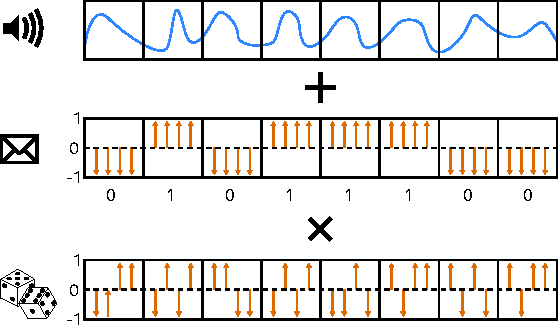
\includegraphics[width=0.8\textwidth]{obrazky/direct-sequence-spread-spectrum-diagram.pdf}
    \caption{Kódování rozprostřených bitů (uprostřed) pomocí metody přímého
    rozprostření spektra vynásobením s~pseudonáhodnou sekvencí (dole)
    a~přidáním ke krycímu signálu (nahoře).}
    \label{pic:dsss-spreading}
\end{figure}

Tato metoda je dostatečně robustní pro přidání více vodoznaků. Například pro
přidání více autorů k~hudební skladbě. Při detekci konkrétního vodoznaku jsou
ostatní považovány jako šum. Dále je tato metoda dostatečně robustní vůči
přidanému šumu a~překódování do ztrátového formátu \cite{Boney1996}. Aby byl
náhodný šum přidaný touto metodou neslyšitelný, je nutné nastavit při kódování
amplitudu rozprostřené sekvence zhruba na 0,5\% dynamického rozsahu krycího
média \cite{Bender1996}. Pro kvalitní dekódování má tato metoda kapacitu 4~bity
za sekundu \cite{Bender1996}.

Pro dekódování informačních bitů je nezbytné, aby příjemce měl stejnou
pseudonáhodnou sekvenci čipů, která byla použita k~zakódování. Pro dekódování
se stego médium a~pseudonáhodná sekvence rozdělí na segmenty a~vypočítá se
korelace mezi každým segmentem stego média a~pseudonáhodné sekvence. Pro určení
hodnoty bitu je možné použít rozhodovací pravidlo v~rovnici
\ref{eq:dsss-decision-rule}, kde $b$ je hodnota bitu a~$c$ je výsledek korelace
\cite{Kuznetsov2022}.

\begin{equation}
    \label{eq:dsss-decision-rule}
    b = \left\{
        \begin{array}{rl}
            0, & c < 0 \\
            1, & c > 0
        \end{array}
    \right.
\end{equation}

\subsection*{Metoda fázového kódování}
\label{sub:phase-coding}

Metoda fázového kódování je založená na nahrazení fáze prvního segmentu audia
referenční fází reprezentující ukrývaná data. Fáze následujících segmentů je
upravena tak, aby byla zachována relativní fáze mezi segmenty. Metoda fázového
kódování dosahuje nejlepších hodnot poměru signálu k~šumu. Avšak příliš velká
změna fáze frekvenční komponenty vede k~rozptylu fáze a~tím ke zhoršení kvality
zvuku. Dokud jsou ale změny fáze dostatečně malé, což je subjektivní, pak je
možné dosáhnout neslyšitelného kódování \cite{Bender1996}.

Kódování pomocí této metody začíná rozdělením krycího audia na segmenty
s~délkou počtu ukrývaných bitů. Poté je každý segment převeden do frekvenční
domény pomocí Fourierovy transformace. Z~transformovaného signálu je možné
vytvořit matici fází -- značeno $\phi_n(\omega_k)$ -- a~matici amplitud
segmentů -- značeno $A_n(\omega_k)$. Písmeno $n$ značí index segmentu a~písmeno
$k$ značí index vzorku uvnitř segmentu. Poté se vypočítá rozdíl fází segmentů
napříč řádky \cite{Bender1996}. Matematický zápis rozdílu fází je v~rovnici
\ref{eq:phase-diff}.

\begin{equation}
    \label{eq:phase-diff}
    \Delta\phi_n(\omega_k) = \phi_{n+1}(\omega_k) - \phi_n(\omega_k)
\end{equation}

\noindent Poté se bity ukrývaných dat převedou do formátu $\frac{\pi}{2}$
reprezentující hodnotu~0 a~$-\frac{\pi}{2}$ reprezentující hodnotu~1. Touto
sekvencí se nahradí první segment v~matici fází. Poté se postupně počítají nové
fáze z~původní fázové matice a~matice rozdílů fází. Matematický zápis je
v~rovnici \ref{eq:new-phases}, kde $\phi'$ značí novou matici fází a~$N$
značí index posledního segmentu \cite{Bender1996}.

\begin{equation}
    \label{eq:new-phases}
    \left[
        \begin{array}{lclcl}
            \phi_1'(\omega_k) & = & \phi_0'(\omega_k)     & + & \Delta\phi_1(\omega_k) \\
            \phi_n'(\omega_k) & = & \phi_{n-1}'(\omega_k) & + & \Delta\phi_n(\omega_k) \\
                              & \vdots \\
            \phi_N'(\omega_k) & = & \phi_{N-1}'(\omega_k) & + & \Delta\phi_N(\omega_k)
        \end{array}
    \right]
\end{equation}

\noindent Na závěr je možné sestavit stego signál z~amplitud a~nových fází
pomocí inverzní Fourierovy transformace \cite{Bender1996}. Z~obou matic je
potřeba zkombinovat hodnoty amplitud a~fází v~jednotlivých segmentech pro
vytvoření komplexních čísel v~exponenciálním tvaru. Na každý segment se poté
aplikuje inverzní Fourierova transformace. Tyto segmenty se znovu spojí
dohromady, čímž vznikne výsledné stego médium. Dekódování probíhá pouhým
převedením fází z~prvního segmentu stego média na bity stejným způsobem jako
při kódování.

Kapacita této metody se pohybuje v~rozsahu 8~bitů za sekundu až 32~bitů za
sekundu podle množství šumu přítomného v~krycím médiu. Více šumu vede k~vyšší
kapacitě \cite{Bender1996}.

\subsection*{Metoda paritního kódování}
\label{sub:parity-coding}

Metoda paritního kódování je založená na ukrývání do nejméně významného bitu
skupiny vzorků na rozdíl od ukrývání do jednotlivých vzorků. Pro zakódování
informace se krycí médium rozdělí na segmenty a~vypočítá se paritní bit
segmentu. Pokud je paritní bit stejný jako informační, pak se neprovádí nic.
Pokud je paritní bit rozdílný, pak se změní nejméně významný bit libovolného
vzorku v~daném segmentu. Díky tomu je možné snížit detekovatelnost informace
\cite{Bandyopadhyay2008}, čímž ale dojde ke snížení robustnosti. Způsob
kódování pomocí této metody je vizualizován na obrázku \ref{pic:parity-coding}.

\begin{figure}[hbt]
    \centering
    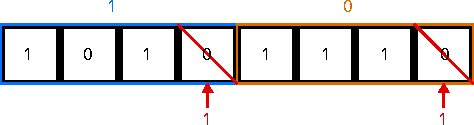
\includegraphics[width=0.8\textwidth]{obrazky/parity-coding.pdf}
    \caption{Metoda paritního kódování. Pro zakódování je potřeba docílit
    stejné parity jako je informační bit.}
    \label{pic:parity-coding}
\end{figure}

\subsection*{Metody založené na nedostatcích lidského sluchového ústrojí}
\label{sub:has}

Tyto metody byly využívány již od počátků steganografie a~využívají percepčních
vlastností lidského sluchového ústrojí a~psychoakustických vlastností řeči.
Tyto metody využívají maskování v~časové nebo frekvenční doméně. Maskování
v~časové doméně využívá nutnosti počkat chvíli po zaslechnutí hlasitého tónu.
Pro ukrytí nějakého tónu je možné vložit jej do bezprostřední blízkosti
hlasitého impulzu. Nápodobně, maskování ve frekvenční doméně probíhá vložením
frekvence, která se nachází v~blízkém okolí nějaké jiné frekvence s~vyšší
amplitudou \cite{Dutta2020}.

Jedna z~metod pracující ve frekvenční doméně je metoda vkládání tónu
\cite{Dutta2020}. Ta spoléhá na neschopnost vnímání tónu v~přítomnosti mnohem
hlasitějších. Pro kódování se krycí médium rozdělí na segmenty a~vypočítá se
výkon každého z~nich. Poté se vloží dva tóny na frekvencích $f_0$ a~$f_1$.
Výkony tónů jsou nastaveny v~předem známém poměru k~výkonu segmentu
\cite{Djebbar2012}. Princip kódování této metody lze vidět na obrázku
\ref{pic:tone-insertion}, kde poměr výkonů tónu na frekvencích $f_0$ a~$f_1$
kóduje bity \texttt{010}.

\begin{figure}[hbt]
    \centering
    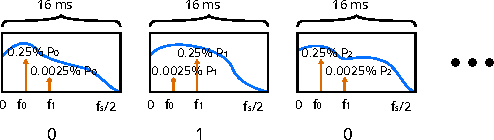
\includegraphics[width=\textwidth]{obrazky/tone-insertion-diagram.pdf}
    \caption{Metoda vkládání tónu. Specifické poměry tónů na frekvencích $f_0$
    a~$f_1$ kódují 0~nebo~1.}
    \label{pic:tone-insertion}
\end{figure}

Dekódování probíhá porovnáním poměrů výkonu segmentu k~výkonu tónu na dané
frekvenci \cite{Djebbar2012}. Dekódovací pravidlo lze vidět v~rovnici
\ref{eq:tone-insertion-decision-rule} kde $b$ značí hodnotu bitu a~výkon
segmentu je označen jako $P_i$ přičemž $i$ značí index segmentu a~$f_0$~a$f_1$
značí použité frekvence.

\begin{equation}
    \label{eq:tone-insertion-decision-rule}
    b = \left\{
        \begin{array}{rl}
            0, & \frac{P_i}{P_{f_0}} > \frac{P_i}{P_{f_1}} \\
            1, & \mathrm{jinak}
        \end{array}
    \right.
\end{equation}

Tato metoda má malou kapacitu a~vložené tóny je jednoduché detekovat, proto je
vhodné použít čtyři a~více párů frekvencí, které se střídají na základě
určitého klíče \cite{Djebbar2012}.

\subsection*{Metoda ukrývání v~úsecích ticha}
\label{sub:hinding-in-silence-intervals}

Tato metoda využívá ke skrývání informací úseky ticha nacházející se
v~nahrávkách řeči \cite{Djebbar2012}. Pro zakódování informací je nejprve
potřeba najít úseky ticha v~nahrávce. Ty se vyskytují jako posloupné sekvence
vzorků s~amplitudou nižší než určitá hodnota. Z~nalezených úseků se ponechají
pouze ty, jejichž délka je větší než minimální délka úseku \cite{Shahreza2008}.
Autoři \cite{Shahreza2008} zjistili následující optimální hodnoty:

\begin{itemize}
    \item maximální amplituda úseku: 15\% maximálního rozsahu signálu,
    \item minimální délka úseku: 200~vzorků; kratší úseky se většinou vyskytují
        mezi částmi slov a~tyto skoky mohou být detekovány,
    \item maximální počet bitů pro ukrytí do segmentu: 4~b.
\end{itemize}

Pokud $X$ je kódovaná hodnota, $N$ je počet bitů kódované hodnoty a~$L$ je
délka konkrétního segmentu, pak pro kódování do konkrétního segmentu se
vypočítá jeho nová délka $D$, tak aby platil vztah v~rovnici
\ref{eq:silence-value} \cite{Shahreza2008}.

\begin{equation}
    \label{eq:silence-value}
    X = D \bmod 2^N
\end{equation}

\noindent Novou délku segmentu lze jednoduše vypočítat z~rovnice
\ref{eq:silence-length}.

\begin{equation}
    \label{eq:silence-length}
    D = L - [(L - X) \bmod 2^N]
\end{equation}

\noindent Pokud by byla nová délka $D$ kratší než je minimální stanovená délka
úseku, pak je potřeba použít jiný úsek. Pro dekódování informace stačí použít
zmíněný vztah \ref{eq:silence-value} \cite{Shahreza2008}.

Nevýhodou této metody je její citlivost na transformaci stego signálu. Změny
délek úseků ticha povedou k~dekódování špatných hodnot. Pro zvýšení robustnosti
v~tomto ohledu je možné snížit amplitudu úseků ticha a~zvýšit amplitudu
okolních úseků, aby nedošlo ke změně délky některého z~úseků například kvůli
kompresi \cite{Djebbar2012}.

\subsection*{Metoda využívající vlnkové transformace}
\label{sub:wavelet-transform}

Nejlepší metodou pro ukrývání informací v~transformační doméně je diskrétní
vlnková transformace (anglicky \textit{discrete wavelet transform} -- DWT),
protože prezentuje informace o~frekvencích, které lze získat z~Fourierovy
transformace jako funkci v~čase. Vlnková transformace poskytuje dobrý kompromis
mezi Fourierovou transformací, která frekvencím nepřiřazuje čas. Další
transformační funkcí je diskrétní kosinová transformace (anglicky
\textit{discrete cosine transform} -- DCT). Ta není pro účely ukrývání
informací příliš vhodná, protože zavádí do audia artefakty. Metody
v~transformační doméně jsou poměrně méně odolné proti šumu \cite{Dutta2020}.

Pro zakódování informace do nosiče se nosič rozdělí na segmenty po
512~vzorcích. Na každý segment je poté pětkrát aplikována dekompozice na
nízkofrekvenční a~vysokofrekvenční komponenty \cite{Cvejic2002Wavelet}. Každá
následující dekompozice je aplikována na nízkofrekvenční složku z~předchozí
úrovně \cite{Prabakaran2012}. Výsledných 512~koeficientů je převedeno na
binární hodnoty do jejichž nejméně významných bitů jsou uloženy bity ukrývané
informace \cite{Cvejic2002Wavelet}. Experimentální výsledky
v~\cite{Cvejic2002Wavelet} ukázaly, že při modifikaci až 7~nejnižších bitů bylo
téměř nemožné rozeznat rozdíl mezi originální a~upravenou nahrávkou. A~i~při
modifikaci více úrovní byly výsledky lepší než při použití konvenční metody
nahrazení nejméně významného bitu popsané v~podsekci \ref{sub:lsb} s~dvakrát
menším počtem upravených bitových úrovní. Tato metoda má velmi vysokou kapacitu
a~je schopna ukrýt až o~220,5\,kb/s více dat než konvenční metoda nahrazení
nejméně významného bitu \cite{Cvejic2002Wavelet}.

Proces dekódování probíhá podobně jako kódování. Stego signál se rozdělí na
segmenty, provede se dekompozice a~koeficienty se převedou na binární hodnoty.
Z~nejnižších bitů je možné vyčíst bity ukryté informace \cite{Pooyan2007}.


\chapter{Analýza a~návrh}
\label{cha:library-design}

V~této kapitole bude popsán konceptuální návrh knihovny a~vestavěného programu
pro zvukovou steganografii a~vysokoúrovňový popis struktury projektu, použitých
technik a~metod k~tvorbě kvalitního a~rozšiřitelného řešení. Budou také popsány
použité softwarové nástroje a~na závěr kapitoly bude popsán princip navrhované
metody pro digitální zvukovou steganografii.

\section{Rozbor řešeného problému}
\label{sec:problem-analysis}

\todo{hodně publikací, nedostatek implementací}

\blindtext

\subsection*{Definice problému}
\label{sub:problem-definition}

\todo{definice problému}

\blindtext

\subsection*{Metody a~prostředky řešení problému}
\label{sub:problem-solution}

\todo{prostředky řešení problému}

\blindtext

\subsection*{Výhody a~nevýhody stávajících řešení}
\label{sub:pros-cons-existing-solutions}

\todo{výhody a nevýhody stávajících řešení}

\blindtext

\section{Návrh řešení}
\label{sec:solution-proposal}

Aby bylo řešení jednoduše rozšiřitelné, bude použit objektově orientovaný
návrh. Každá ze steganografických metod bude mít společné rozhraní, aby bylo
použití a~implementace nových metod co nejjednodušší. Dalším požadavkem na
řešení je, aby bylo čitelné a~jednoduše pochopitelné.

Při volbě tajné zprávy bude mít uživatel programu na výběr textový vstup nebo
obsah souboru. Rozhraní jednotlivých metod bude pracovat s~bity ukrývané
informace, díky čemu nebude nezáležet na typu kódovaných dat. Pro kódování je
tedy postačí převést z~bytů na bity a~při dekódování naopak.

Z~metod popsaných v~sekci~\ref{sec:existing-methods} jsem se rozhodl
implementovat všechny, kromě metody vlnkové transformace, protože je velmi
složitá a~také metody paritního kódování, protože se jedná prakticky
o~modifikaci metody nahrazení nejméně významného bitu. U~vybraných budou
implementovány také některé popsané modifikace metod.

\subsection*{Blokové schéma a~komponenty systému}
\label{sub:solution-components}

Struktura řešení se bude skládat z~několika modulů a~balíčků. Pro zjednodušení,
modul je jeden soubor a~balíček je kolekce modulů. Jádrem knihovny bude balíček
s~moduly implementovaných metod pro digitální zvukovou steganografii. Druhý
hlavní balíček bude obsahovat moduly týkající se vestavěného programu
s~terminálovým rozhraním. Nejdůležitějším modulem pro programovou část bude
modul s~fasádou, která zjednoduší volání jednotlivých metod při použití
z~terminálu. Bude také poskytovat výpočty různých statistických funkcí na
základě kterých bude možné vyhodnotit pro konkrétní krycí soubor úroveň
jednotlivých vlastností steganografických metod popsaných v~sekci
\ref{sec:method-properties}. Blokové schéma popsané struktury je možné vidět na
obrázku \ref{pic:library-block-diagram}.

\begin{figure}[hbt]
    \centering
    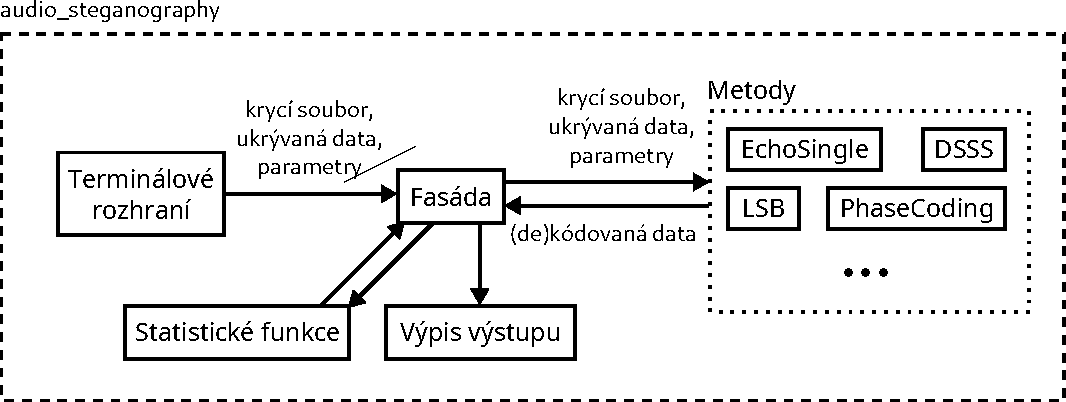
\includegraphics[width=\textwidth]{obrazky/block-diagram.pdf}
    \caption{Blokové schéma knihovny pro digitální zvukovou steganografii}
    \label{pic:library-block-diagram}
\end{figure}

\subsection*{Realizační prostředky a~metody}
\label{sub:solution-tool-choices}

K~implementaci navrženého řešení jsem zvolil programovací jazyk \textit{Python}
minimální verze~\textit{3.8}. Tento jazyk jsem vybral, protože je to
vysokoúrovňový jazyk s~dobře čitelnou syntaxí. Je také dynamicky typovaný
a~umožňuje kombinovat objektově orientovaný a~funkcionální styl programování,
díky čemu je možné psát elegantní kód. Další kvalitou je dobré rozhraní
s~jazykem~\textit{C}, díky kterému mohou být knihovny velmi rychlé. Jednou
takovou knihovnou je knihovna \textit{NumPy}\footnote{https://numpy.org}, která
poskytuje optimalizované funkce pracující s~vícedimenzionálním polem jménem
\textit{NDArray}. Na této datové struktuře a~funkcích staví celá řada dalších
numerických knihoven, jako například knihovna
\textit{SciPy}\footnote{https://scipy.org}, která pomocí NumPy implementuje
velké množství funkcí pro účely zpracování signálů.

\subsection*{Případy užití}
\label{sub:use-cases}

Program bude umožňovat uživateli zvolit steganografickou metodu a~pomocí ní
zakódovat a~dekódovat tajnou zprávu ve formě textu nebo souboru.

\subsection*{Ověřování vlastností}
\label{sub:method-property-verification}

Pro ověření vlastností steganografických metod bude součástí knihovny druhý
vestavěný program, který bude systematicky testovat jednotlivé vlastnosti každé
metody. Testování bude probíhat na často používaných datových sadách pro
digitální zvukovou steganografii. Podle \cite{AlSabhany2020} jsou to tyto
datové sady: \textit{TIMIT} \cite{Garofolo1993}, \textit{GTZAN}
\cite{Tzanetakis2001}, \textit{Noizeus} \cite{Hu2006} a~\textit{UrbanSound8K}
\cite{Salamon2014}.

Hodnoty jednotlivých vlastností se vyčíslují pomocí statistických funkcí, které
se často objevovaly v~průzkumu \cite{AlSabhany2020}. Tyto funkce jsou:

\begin{itemize}
    \item poměr signálu k~šumu měřen v~decibelech (anglicky
        \textit{signal-to-noise ratio}, dále jen SNR),
    \item špičkový poměr signálu k~šumu měřen v~decibelech (anglicky
        \textit{peak signal-to-noise ratio}, dále jen PSNR),
    \item míra bitové chybovosti (anglicky \textit{bit error rate}, dále jen
        BER),
    \item střední kvadratická chyba (anglicky \textit{mean squared error}, dále
        jen MSE)
    \item směrodatná odchylka (anglicky \textit{root-mean-square deviation},
        dále jen RMSD)
\end{itemize}

Rovnice těchto funkcí jsou v~příloze~\ref{cha:statistical-functions}. Při
testování se nejprve vyhodnotí maximální kapacita metody bez modifikace stego
signálu s~pomocí funkce BER. Poté bude testována robustnost následujícími
metodami zvlášť i~kombinovaně:

\begin{itemize}
    \item přidání šumu,
    \item filtrace spektra,
    \item převzorkování,
    \item překvantování,
    \item překódování do ztrátového formátu.
\end{itemize}

Nepostřehnutelnost je sice subjektivní vlastnost, ale je možné částečně
vyhodnotit její míru automaticky pomocí úrovně SNR a~PSNR.

\section{Popis vlastní metody digitální zvukové steganografie}
\label{sec:own-method-proposal}

\todo{popis vlastní metody}

\blindtext

\blindtext


\definecolor{backcolor}{rgb}{0.95,0.95,0.92}
\definecolor{codegreen}{rgb}{0,0.6,0}
\definecolor{codegreen2}{rgb}{0,0.6,0.2}
\definecolor{codepurple}{rgb}{0.6,0,0.6}
\definecolor{codeorange}{rgb}{0.8,0.2,0}
\lstdefinestyle{mystyle}{%
    showspaces=false,
    showtabs=false,
    breaklines=true,
    showstringspaces=false,
    breakatwhitespace=true,
    escapeinside={(*@}{@*)},
    backgroundcolor=\color{backcolor},
    commentstyle=\color{codegreen},
    keywordstyle=\color{codepurple},
    keywordstyle=[2]\color{darkblue},
    keywordstyle=[3]\color{codepurple},
    keywordstyle=[4]\color{codegreen2},
    stringstyle=\color{codeorange},
    basicstyle=\ttfamily,
    captionpos=b,
    numbers=left,
    frame=single,
    numberstyle=\tiny,
    aboveskip=1em,
    abovecaptionskip=6pt,
}%
\lstset{style=mystyle}%
\lstdefinelanguage{PythonPlus}[]{Python}{%
    morekeywords=[1]{,as,assert,nonlocal,with,yield},
    morekeywords=[2]{,self,True,False,None,},
    morekeywords=[4]{,ValueError},
}%

% \begin{lstlisting}[language=PythonPlus, label={lst:}, caption={}]
% \end{lstlisting}

\chapter{Realizace systému}
\label{cha:implementation}

\todo{popis kapitoly implementace}

\blindtext

\section{Struktura modulů knihovny}
\label{sec:modules}

\todo{popis modulů knihovny}

\blindtext

\blindtext

\blindtext

\section{Implementace metod}
\label{sec:method-implementation}

\subsection*{Metoda nahrazení nejméně významného bitu}
\label{sub:lsb-implementation}

\blindtext

\subsection*{Metoda skrývání pomocí ozvěny}
\label{sub:echo-hiding-implementation}

\blindtext

\subsection*{Metoda rozprostřeného spektra}
\label{sub:dsss-implementation}

\blindtext

\subsection*{Metoda fázového kódování}
\label{sub:phase-coding-implementation}

\todo{popis metody fázového kódování}

\blindtext

\subsection*{Metoda paritního kódování}
\label{sub:parity-coding-implementation}

\todo{popis metody paritního kódování}

\blindtext

\subsection*{Metody založené na nedostatcích lidského sluchového ústrojí}
\label{sub:has-implementation}

\todo{popis metody HAS}

\blindtext

\subsection*{Metoda využívající vlnkové transformace}
\label{sub:wavelet-transform-implementation}

\todo{popis wavelet metody}

\blindtext


\chapter{Zhodnocení vlastností realizace}
\label{cha:method-evaluation}

\todo{výsledky vyhodnocení kvality}

\blindtext

\blindtext

\begin{figure}[hbt]
    \centering
    
\includegraphics[width=0.3\textwidth]{obrazky/placeholder.pdf}
    \caption{Placeholder}
    \label{pic:placeholder}
\end{figure}

\blindtext

\begin{figure}[hbt]
    \centering
    
\includegraphics[width=0.3\textwidth]{obrazky/placeholder.pdf}
    \caption{Placeholder}
    \label{pic:placeholder}
\end{figure}

\blindtext

\blindtext

\blindtext

\begin{figure}[hbt]
    \centering
    
\includegraphics[width=0.3\textwidth]{obrazky/placeholder.pdf}
    \caption{Placeholder}
    \label{pic:placeholder}
\end{figure}

\blindtext

\blinditemize

\blindtext

\blindtext

\blinditemize

\blindtext

\begin{figure}[hbt]
    \centering
    
\includegraphics[width=0.3\textwidth]{obrazky/placeholder.pdf}
    \caption{Placeholder}
    \label{pic:placeholder}
\end{figure}

\blindtext

\blindtext

\chapter{Závěr}
\label{cha:conclusion}

\blindtext

\blindtext

\blindtext
